% mn2esample.tex
%
% v2.1 released 22nd May 2002 (G. Hutton)
%
% The mnsample.tex file has been amended to highlight
% the proper use of LaTeX2e code with the class file
% and using natbib cross-referencing. These changes
% do not reflect the original paper by A. V. Raveendran.
%
% Previous versions of this sample document were
% compatible with the LaTeX 2.09 style file mn.sty
% v1.2 released 5th September 1994 (M. Reed)
% v1.1 released 18th July 1994
% v1.0 released 28th January 1994

\documentclass[useAMS,usenatbib]{mn2e}
\usepackage{graphics}
\usepackage{epsfig}

\voffset-1.25cm

% If your system does not have the AMS fonts version 2.0 installed, then
% remove the useAMS option.
%
% useAMS allows you to obtain upright Greek characters.
% e.g. \umu, \upi etc.  See the section on "Upright Greek characters" in
% this guide for further information.
%
% If you are using AMS 2.0 fonts, bold math letters/symbols are available
% at a larger range of sizes for NFSS release 1 and 2 (using \boldmath or
% preferably \bmath).
%
% The usenatbib command allows the use of Patrick Daly's natbib.sty for
% cross-referencing.
%
% If you wish to typeset the paper in Times font (if you do not have the
% PostScript Type 1 Computer Modern fonts you will need to do this to get
% smoother fonts in a PDF file) then uncomment the next line
% \usepackage{Times}

%%%%% AUTHORS - PLACE YOUR OWN MACROS HERE %%%%%

%\newcommand{\Mvir}{$\rm M_{\rm vir}$}
%\newcommand{\Rvir}{$\rm R_{\rm vir}$}
%\newcommand{\cvir}{$\rm c_{\rm vir}$}
%\newcommand{\Ms}{$\rm M_{\rm s}$}
%\newcommand{\rs}{$\rm r_{\rm s}$}

%\newcommand{\hMpc}{$h^{-1}\rm{Mpc}$}
%\newcommand{\hMsun}{$\rm {M_{\odot}h^{-1}}$}

\newcommand{\Rq}{$\rm R_{1/4} $}
\newcommand{\etal}{et al.~}
\newcommand{\rhocrit}{\rho_c}
\newcommand{\rhorms}{\rho_{\rm rms}}
\newcommand{\xoff}{x_{\rm off}}
\newcommand{\cvir}{c_{\rm vir}}
\newcommand{\Rvir}{R_{\rm vir}}
\newcommand{\Mvir}{M_{\rm vir}}
\newcommand{\rs}{r_{\rm s}}
\newcommand{\Jvir}{J_{\rm vir}}
\newcommand{\Vvir}{V_{\rm vir}}
\newcommand{\Nvir}{N_{\rm vir}}
\newcommand{\Ms}{M_{\rm s}}

\def \kms {\ifmmode  \,\rm km\,s^{-1} \else $\,\rm km\,s^{-1}  $ \fi }
\def \kpc {\ifmmode  {\rm kpc}  \else ${\rm  kpc}$ \fi  }  
\def \Msun {\ifmmode M_{\odot} \else $M_{\odot}$ \fi} 
\def \hMsun {\ifmmode h^{-1}\,\rm M_{\odot} \else $h^{-1}\,\rm M_{\odot}$ \fi}
\def \hMpc {\ifmmode h^{-1}\,\rm Mpc \else $h^{-1}\,\rm Mpc$ \fi}
\def \hkpc {\ifmmode h^{-1}\,\rm kpc \else $h^{-1}\,\rm kpc$ \fi}
\def \hLsun {\ifmmode h^{-1}\,\rm L_{\odot} \else $h^{-1}\,\rm L_{\odot}$ \fi}

\newcommand{\mnras}{MNRAS}
\newcommand{\apj}{ApJ}
\newcommand{\apjl}{ApJ}
\newcommand{\apjs}{ApJS}
\newcommand{\aj}{AJ}
\newcommand{\aap}{A\&A}
\newcommand{\nat}{Nature}

%%%%%%%%%%%%%%%%%%%%%%%%%%%%%%%%%%%%%%%%%%%%%%%%

\title[Are local group galaxies so improbable?]
{Are local group galaxies so improbable?}
\author[J. C. Mu\~noz-Cuartas, et al.]
{fulano, perano mengano. Disc survival collaboration UdeA-AIP$^{1}$$^{2}$\\
$^{1}$ Leibniz-Institut F\"{u}r Astrophysik Potsdam, An der Sternwarte 16, 14482
Potsdam, Germany.\\
$^{2}$ Instituto de Fisica, Universidad de Antioquia, Medellin, Colombia.
}
\begin{document}

\date{Accepted XXXX December XX. Received XXXX December XX; in original form
  2009 June 27}

\pagerange{\pageref{firstpage}--\pageref{lastpage}} \pubyear{2002}

\maketitle

\label{firstpage}

\begin{abstract}
  


\end{abstract}

\begin{keywords}
galaxies: haloes, groups -- cosmology: dark matter, observations
\end{keywords}



%%%%%%%%%%%%%%%%%%%%%%%%%%%%%%%%%%%%%%%%%%%%%%%%%%%%%%%%%%%%%%%%%%%%%%%
%%%%%%%%%%%%%%%%%%%%%%%%%%%%%%%%%%%%%%%%%%%%%%%%%%%%%%%%%%%%%%%%%%%%%%%

\section{Introduction}

cosmological scenario
the local group
the problem of locating the LG in the universe

The questions we want to address in this paper is: How common is the
local group of galaxies in the cosmological context? what is the
probability of generate a local group in the universe? under which
physical conditions do we reproduce the properties of the local group?


%%%%%%%%%%%%%%%%%%%%%%%%%%%%%%%%%%%%%%%%%%%%%%%%%%%%%%%%%%%%%%%%%%%%%%
%%%%%%%%%%%%%%%%%%%%%%%%%%%%%%%%%%%%%%%%%%%%%%%%%%%%%%%%%%%%%%%%%%%%%%


\section{Methods} 
\label{sec:method}

\subsection{N-body simulations}
\label{sec:simul}

In this work we study the evolution of galaxies in the local universe
through the use of semi-analytic models of galaxy evolution. To
properly constrain the study to the local group it is required to use
then constrained simulations of the local universe. A constrained
simulation of the local universe is a standard N-body simulation of
the formation of structure in which observational constraints have
been imposed in order to reproduce the large scale environment of the
local universe (Martinez-Vaquero \etal 2009, Gottloeber \etal 2010,
Doumler \etal 2012).

The constrained simulations used in this work are part of a suite of
cosmological simulations part of the CLUES (Constrained Simulations of
the Local Universe) project (Gottloeber \etal 2010). The observational
constraints impose conditions on the large scale structure of the local
universe on scales above a few mega parsec, however the small scales
keep unconstrained and behave basically randomly. In order to overcome
this problem, and to get a realisation that matches as close as
possible not only the large scale environment but also the environment
of the local group, many realisations are required of the same piece
of the universe with the same constraints. From this set of
realisations (200 in the case of the CLUES) a few have been selected
to be potential candidates in which not only the large scale
environment but also the small scale environment have been reproduced.

The criteria used to identify fiducial local group realisations are

\begin{itemize}
\item
\item
\item
\end{itemize}

From a set of 200 low resolution simulations, three satisfy the
criteria imposed. These three simulations are the re run at high
resolution keeping the constrain on the large scale structure.

The final set of simulations we have used in this work is then a set
of three simulations with a box size of 64 \hMpc and sampled with
$1024^3$ particles giving a particle mass is $1.09\time10^7$
\hMsun. The candidates to milky way and Andromeda galaxy in these
simulations are resolved with more than XXXX particles. The starting
redshift of the simulation was 50, and it was run with the
cosmological Tree-PM code Gadget-2 (Springel 2005).

The use of the constrained simulations provide us with the unique
opportunity to model the large and small scale environment of the local
group, and pick candidate objects to host the milky way and Andromeda
galaxy. Simultaneously, the realisation of simulations of dark matter
only provide us with the opportunity to simulate a fairly large sample
of galaxies. For each of the three simulations we have around XXX
haloes, and XXX haloes in the mass range XXX to XXX. In general,
combining the three data sets we have a total of ~27000 haloes in the
mass range of XXX to XXX, which provide us with a large statistical
sample of MW type haloes.

Merger trees ........

\subsection{Semi-analytic Modelling} 
\label{sec:sam}

description of galacticus and the recipes we use

Since the simulations we have performed are dark matter only, galaxy
formation has to be modelled as an external process happening inside
dark matter haloes. One of the advantages of using this semi-analytic
approach is the opportunity to explore the parameter space and to find
the parameter set that best reproduce the observed structure of the
local group galaxies.

Instead of developing our own semi-analytic code we opted for the
alternative to use a publicly available semi-analytic code for galaxy
formation. The code we used in this work is GALACTICUS. A
semi-analytic code developed by Andrew Benson (Benson
2011). GALACTICUS implements several physical processes and implements
different approaches for each different process. Instead of exploring
the many different possibilities of the code, we keep close to the
``basic'' usage of the code, used standard recipes to model the
different physical processes.

In our simulations we have included many different physical phenomena:
bla, bla, blahhh.

Each physical process is controlled by one or more parameters. From
those processes we detail the most important ones, those are the ones we
have decided to vary in order to explore the parameter space
associated with the probability of having a local group.

\subsubsection{Galaxy mass growth}

One would expect that the accretion of cold gas in a dark matter halo
depends on the growth rate of mass of the halo, but also on the
available gas mass, the mass of the halo itself and the
thermodynamical conditions of the gas. In GALACTICUS we use the {\em
  simple} method to model the accretion of cold gas like

\begin{equation}
 \dot{M}_{{\rm accr}}=
 \begin{cases}
   (\Omega_b/\Omega_M)\dot{M}_{{\rm halo}},\quad {\rm if} \quad V_{{\rm virial}}>V_{{\rm reioniz}}\\
   \qquad \qquad \qquad \qquad {\rm or} \quad z>z_{{\rm reioniz}}\\
0, {\rm otherwise}
\end{cases}
\end{equation}

where $\Omega_b/\Omega_M$ is the cosmic baryon fraction that basically
controls the amount of available baryons and $V_{\rm reioniz}$ and
$z_{\rm reioniz}$ are the free parameters that model cold gas
accretion. If a halo has a low velocity (lower than the threshold
$V_{\rm reioniz}$) is not massive enough to accrete and keep cold
gas. Also, if the redshift is larger than $z_{\rm reioniz}$ the
temperature of the gas should be high enough and no effective cooling
should be present.


\subsubsection{star formation time scale}

We have used the standard Cole \etal 2000 star formation time
scale. It is parameterized by a power law in the halo velocity

\begin{equation}
 \tau_{\star} = \epsilon^{-1}_{\star}\tau_{{\rm dyn}}\left(
 \frac{V}{200{\rm km/s}}\right)^{\alpha_\star}
\end{equation}

with free parameters $\epsilon_{\star}$ and $\alpha_\star$ that control
the star formation efficiency and the shape on the velocity (or mass)
dependence of the star formation time scale.

\subsubsection{supernova feedback}

Mass ejection from supernovae is modeled as

\begin{equation}
 \dot{M}_{\rm outflow}=\left( \frac{V_{\rm outflow}}{V}
 \right)^{\alpha_{\rm outflow}}\frac{\dot{E}}{E_{\rm canonical}}, \label{eq:supernovae}
\end{equation}

where $V_{\rm outflow}$ is a threshold velocity for the galactic
component. The larger the value of $V_{\rm outflow}$ the stronger the
suppression of the outflow of mass. The second parameter is
$\alpha_{\rm outflow}$, and as $\alpha_\star$ controls the mass
dependence of the outflow. $V$, $\dot{E}$ and $E_{\rm canonical}$ are
not constants, they are the velocity of the component, the rate of
energy input from the stellar populations and the energy input by a
stellar population normalised to $1 {\rm M}_{\odot}$ after an infinite time.

\subsubsection{Minor/Mayor merger ($\eta$)}

We define a minor merger between a massive halo $M_{Hm}$ and a low
mass halo $M_{Lm}$ if

\begin{equation}
\frac{M_{Lm}}{M_{Hm}} \leq \eta
\end{equation}

in other case the merger will represent a major merger.

\subsubsection{Merger mass flow}

After a merger (minor or major) the mass of the galaxies must be
redistributed in the remnant. The way the mass is redistributed in the
remnant depends on the characteristics of the merger.

\begin{itemize}

\item
If the merger is a major merger the structure of both galaxies is
destroyed and all mass from both galaxies moves to the spheroid of the
remnant central galaxy.

\item
In the case of a minor merger the mass of the satellite moves to the
component that is indicated by the respective flag. $M_{{\rm
    satel.,gas}}\to$, where in our case gas and stars can move from
the satellite to the disk or to the bulge of the central galaxy.

\end{itemize}


\subsubsection{galaxy structure: Spin and concentration parameter}

The structural properties of the galaxy depend partially on the
structural properties of the dark matter halo. We used the approach
included in GALACTICUS that allows to use the fitting formulas of
Prada \etal 2011 to model the concentration parameter of halos as a
function of mass and redshift while for the spin parameter used two
prescriptions. The first one is the fitting formula from Bett \etal
2007. The second prescription assumes that the spin parameter follows
a lognormal distribution with mean $\mu_{\lambda} = 0.031$ and
variance $\sigma_{\lambda} = 0.57$ as computed from cosmological
simulations by Mu\~noz-Cuartas \etal (2011).


\subsection{Observational samples and definition of our local group}
\label{sec:LGdefine}

describe the data sample used to define the local group

We have already shown how we define the milky way and Andromeda
galaxies in our simulations. Now we need to introduce an operational
definition for these galaxies from the observational point of
view. Clearly, MW and Andromeda are characterised by its observational
properties. Considering the quantities we can reliably model using the
semi-analytic approach. We will define, or characterise the milky way
galaxy and Andromeda.\\

\begin{table}
\centering
\begin{tabular}{|l|l|l|l|l|}
\hline
\hline
 Property &  MW &  Ref. & M31 & Ref.\\
\hline
$M_{disk,\star}[10^{10}M_{\odot}]$ & $3.0 $ &  $(1)$ & $7.2$ & $(2)$ \\
$M_{disk,gas}[10^{10}M_{\odot}]$ & $0.7$ &  $(3)$ & $0.6$ &  $(4)$ \\
$M_{bulge,\star}[10^{10}M_{\odot}]$ & $1-2$ & $(3)$ & $3.2$ &  $(2)$ \\
$V_{circ}[{\rm Km/s}]$ & $238$ &  $(5)$ & $275\pm 5$ & $(6)$ \\
%& $220$ & $(7)$ &   &  \\
%$r_d[\text{Kpc}]$ & $2.38$ & $(5)$  & $5.48$ & $(3)$  \\
 %&  $3.7\pm 1$ &  & ...  \\
\hline
\hline
\end{tabular}
\caption{Observational estimations for different properties of the LG, where$(1)$\citet{2001ApJ...555..393Z},
$(2)$ \citet{2006MNRAS.366..996G}, $(3)$\citet{2009A&A...505..497Y}, $(4)$ \citet{2006A&A...453..459N}, $(5)$\citet{2005MNRAS.364..433B}, 
$(6)$\citet{2008MNRAS.389.1911S}.
}
\label{tab:lg-observations}
\end{table}


We decide to define the Milky Way and Andromeda galaxies through
XXXXX, XXXXX, XXXXX, and XXXX because XXXXX, XXXXX and XXXX.

{\bf Disk stellar mass}. The principal approach to estimate the
stellar mass in the disk of our galaxy is dynamical modelling. The
work of \cite{Klypin2002} uses a parametric model that does not
distinguish between the cold (gas) co component and the stars, their
results for galaxy models that allow for exchange of angular momentum
locate the total baryonic mass of the disk between $5-6\times
10^{10}$\Msun for the MW and $7-9\times 10$\Msun for M31. Later
\cite{Widrow2005} use N-body realisations of self-consistent,
equilibrium distributions of the dark matter and stellar components to
address the same problem. Their models with good match to the
observational data have stellar masses of $3.3-4.5\times 10^{10}$\Msun
for the Milky Way and $7-10\times 10^{10}$ for
Andromeda. \citep{Geehan2006} modeled the Andromeda strem using
analytic bulge-disc-halo for M31, finding the best agreement for a
disk mass of $8.4\times 10^{10}$\Msun. In this work we take
$3.3-4.5\times 10^{10}$\Msun for the Milky Way and $7-10\times
10^{10}$ for M31.

{\bf Bulge stellar mass}. \cite{Klypin2002} constrain the MW bulge
stellar masss $1-1.2\times 10^{10}$ \Msun while for M31 $1.9-2.4\times
10^{10}$, for the same galaxy \citep{Geehan2006} find a bulge mass of
$3.3\times 10^{10}$\Msun. The MW analytical model of model
\citep{Dehnen1998} finds a range of different values with average
$\sim 0.5 10^{10}$\Msun. In this work we pick $0.5-1.2 \times
10^{10}$\Msun for the MW and $1.9-3.3\times 10^{10}$\Msun for M31.

{\bf Disk Gaseous mass}. The abundance of gas in the Milky Way has
been constrained through chemical evolution models. The set of
observational constraints on these models most notably include the gas
and star formation rate (SFR) profiles. The relevant observational
data was compiled in \citep{Boissier99} using from the original work
in \cite{Kulkarni87,Dame93}, with a values of $6.0-8.0 \times
10^{9}$\Msun, an update implementation of this chemical evolution
model by \citep{Yin09} uses the same observations. In the case of M31
the best observational constraints come from the observations by
\citep{Cram80} with the integrated mass of neutral gas corrected by
\citep{Dame93}, yielding a value of $5.2\times 10^{9}$\Msun, there is
a systematic observational uncertainty of $5\%$ originally quoted in
\citep{Cram80}, but due to opacity effects of the HI \citep{Braun92}
the total value of gas can increase by a $19\%$. Therefore we keep a
value of $5.0-6.0\times 10^{9}$ for the mass of gas in the M31 disk
and $6.0-8.0\times 10^{9}$\Msun for the Milky Way.


\subsection{Analysis strategy}
\label{sec:strategy}

Introduce the metric and technique used to quantify the distance and
probability of MW.

\begin{table*}
\centering
%\resizebox{7in}{!} {
\begin{tabular}{|l|l|l|l|l|l|l|l|l|}
\hline
\hline
Model  &  $z_{reioniz}$ &  $M_{{\rm satel.,gas}}\to$  & $\eta$ & $P(\lambda)$  &  $\mu_\lambda$
 & $\sigma_\lambda$  & $\alpha_{{\rm disk,outflow}}$ & $\epsilon_{{\rm disk},\star}$ \\
\hline
\hline
%\\[0pt]
R1 & 9.0 &  bulge & 0.3 &Bett 2007 & &  & 2.0 & 0.01 \\
%run-v2 & 7.0 &  bulge & 0.3 &Lognormal & 0.03687 & 0.2216 & 2.0 & 0.01 \\
R2 & 7.0 &  bulge & 0.3 &Lognormal & 0.031 & 0.57 & 2.0 & 0.01 \\
R3 & 7.0 &  disk & 0.3 &Lognormal & 0.031  & 0.57 & 2.0 & 0.01 \\
\hline
E1 & 7.0 &  disk & 0.3 &Lognormal & 0.031 & 0.57 & 2.0 & 0.02 \\
E2 & 7.0 &  disk & 0.3 &Lognormal & 0.031 & 0.57 & 2.0 & 0.035 \\
E3 & 7.0 &  disk & 0.3 &Lognormal & 0.031 & 0.57 & 2.0 & 0.05 \\
E4 & 7.0 &  disk & 0.3 &Lognormal & 0.031 & 0.57 & 2.0 & 0.075 \\
E5 & 7.0 &  disk & 0.3 &Lognormal & 0.031 & 0.57 & 2.0 & 0.1 \\
\hline
A1 & 7.0 &  disk & 0.3 &Lognormal & 0.031 & 0.57 & 1.5 & 0.01 \\
A2 & 7.0 &  disk & 0.3 &Lognormal & 0.031 & 0.57 & 2.5 & 0.01 \\
A3 & 7.0 &  disk & 0.3 &Lognormal & 0.031 & 0.57 & 3.0 & 0.01 \\
\hline
D1 & 7.0 &  disk & 0.2 &Lognormal & 0.031 & 0.57 & 2.0 & 0.01 \\
D2 & 7.0 &  disk & 0.4 &Lognormal & 0.031 & 0.57 & 2.0 & 0.01 \\
\hline
B1 & 7.0 &  bulge & 0.2 &Lognormal & 0.031 & 0.57 & 2.0 & 0.01 \\
B2 & 7.0 &  bulge & 0.4 &Lognormal & 0.031 & 0.57 & 2.0 & 0.01 \\
\hline
\hline
\end{tabular}
%}
\caption{Set of four experiments intended to model the galaxies hosted
  in halos of mass range of $11.0<log_{10} M_{{\rm
      DM}}<13.0$.}
\label{tab:runs}
\end{table*}


Our goal is to determine quantitatively (instead of qualitatively)
which is the probability to find a galaxy like the milky way and
Andromeda in a given cosmological volume, as well as to see which are
the values of the parameters in the model that maximise the
probability of finding such a galaxies.

To do so we have already defined what a milky way would be, but we
need to quantify how far are our models from such a definition, and
from this distance, we can quantify the probability of finding milky
way like galaxies in the nearby universe.

We define the distance between two galaxies (the defined MW and the
model galaxy) through the distance measure

\begin{equation}
  d = \sqrt{ \sum_{i=1}^N \left( \frac{y_i - m_i}{\sigma_i} \right)^2
  }
  \label{eq:distance}
\end{equation}

The distance $d$ indicates the actually the distance measure (or
difference) between two points in a space defined by the parameter set
$m_i$. the parameter set $m_i$ is the set of values of quantities
associated with the definition of our milky way and Andromeda
galaxies, that is, stellar mass, circular velocity, XXXX, XXXX and
XXXX. the values $y_i$ are the values associated with those parameters
for each model galaxy in our simulations. $sigma_i$ is the error
associated with the estimated value of the observed parameter $m_i$
which will be in any case larger than the uncertainty one can associate
with the values of the parameters in the model galaxy.

One can clearly notice that so defined, $d$ should follow a chi-square
distribution, since it is defined in an equivalent way. Without loss
of generality in our context this quantity can be associated to a
measure distance more than the normal interpretation (Press \etal
XXXX) of it as an estimation of goodness of fit. Another advantage is
that so defined, assuming that the parameters $m_i$ are independent,
$d$ should be distributed following a chi-square distribution, which
will help us to interpret our results in a probabilistic way.

We then compute the value of the distance $d$ from each model galaxy
to the defined galaxies MW and Andromeda and trough it examine
quantitatively the probability to find such an object in our
simulations.


%%%%%%%%%%%%%%%%%%%%%%%%%%%%%%%%%%%%%%%%%%%%%%%%%%%%%%%%%%%%%%%%%%%%%%%
%%%%%%%%%%%%%%%%%%%%%%%%%%%%%%%%%%%%%%%%%%%%%%%%%%%%%%%%%%%%%%%%%%%%%%%

\section{Results}
\label{sec:results}

Now we present the results of our research. Since we are interested in
to find Milky Way and Andromeda like galaxies, we will ignore all
very massive and very low mass objects, and will focus only in a mass
range around the estimated halo mass of those objects

\subsection{Verification tests}

We show that the SAM and our tress and simulations reproduce the
trends.

A first test one should make is to see if our simulation, our post
processing and merger tree constructions as well as the semi-analytic
method are able to reproduce the basic observables on the distribution
of galaxies.

To do so we have just run GALACTICUS on out three boxes and compute
the colour magnitude diagram and the I-band Tully-Fisher fisher relation.

In Figure \ref{fig:T-F-diagram} we show the I-band Tully-Fisher
relation. The data point are from Pizzano \etal (2007). The lines show
the median value for the relation we obtain fro the runs R1, R2 and
R3, where we have used the reference parameter values of GALACTICUS
modifying only the redshift of reionization and the distribution of
spin parameter. With the same simulations we have performed the
comparison of the colour magnitude diagram obtained in our simulations
with the data of the SDSS shown in Mu\~noz-Cuartas \& Mueller
2012. The gray region shows the data from SDSS while the lines show
the median values obtained from the model galaxies in our three boxes.
As it can be seen, GALACTICUS can reproduce quite well obervables
using our data, which give us confidence about the procedures
implemented in the code and in the techniques we used to post analyse
our N-body simulations.


\begin{figure}
 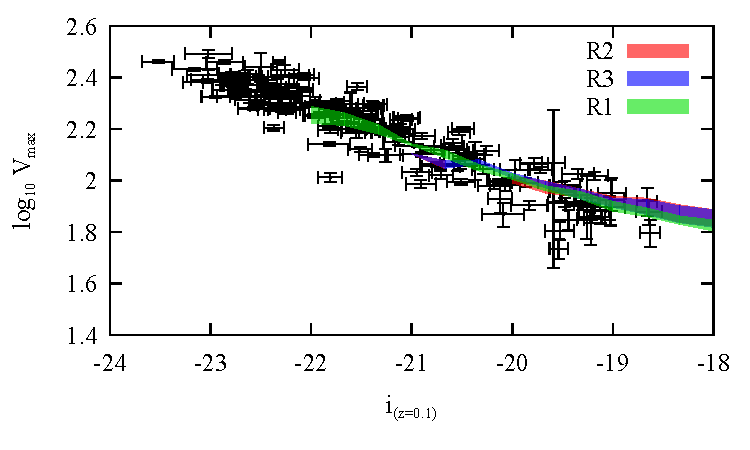
\includegraphics[scale=0.68, angle=0]{figures/tests/T_F-disk-velmax.pdf}
\caption{ Tully-Fisher  relation. The magnitudes where calculated
  without dust extinction and the parameters of the models can be seen
  at Table \ref{tab:runs} as R1, R2 and R3. The error bars correspond
  to the results of \citet{2007AJ....134..945P}.}
\label{fig:T-F-diagram}
\end{figure}


\begin{figure}
 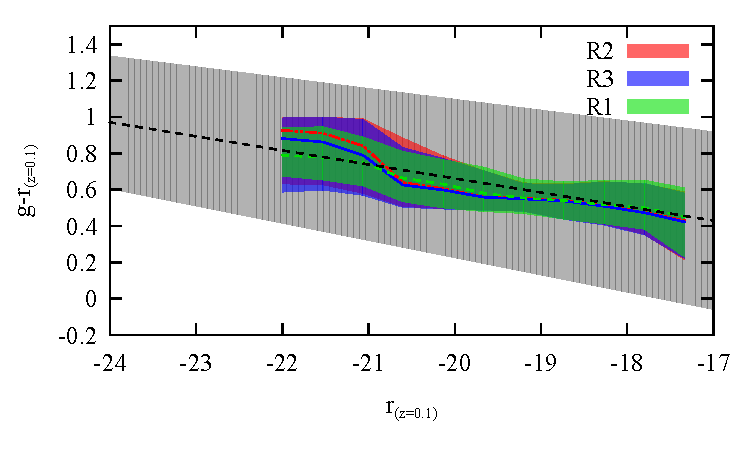
\includegraphics[scale=0.68,angle=0]{figures/tests/Color_Mag.pdf}
\caption{ Colour magnitude relation. Magnitudes were calculated without
  extinction. This is the reference simulation presented in table
  \ref{tab:runs} as R1, R2 and R3. The shaded region correspond to a
  scatter of $2\sigma$ from the work of
  \citet{2012MNRAS.423.1583M}.\label{fig:CM-diagram}}
\end{figure}


\subsection{Searching Local group galaxies}

\begin{figure}
 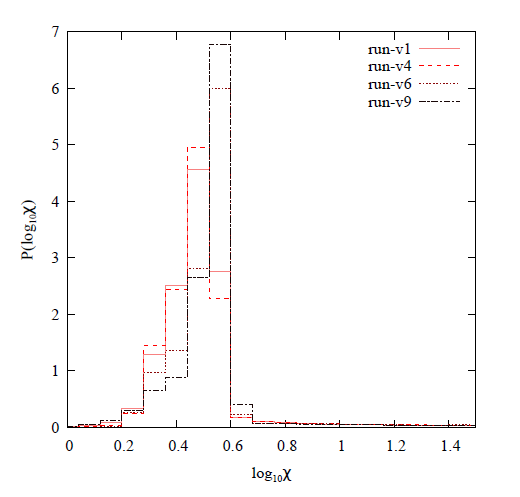
\includegraphics[scale=0.4,angle=0]{figures/fig4_old.png}
 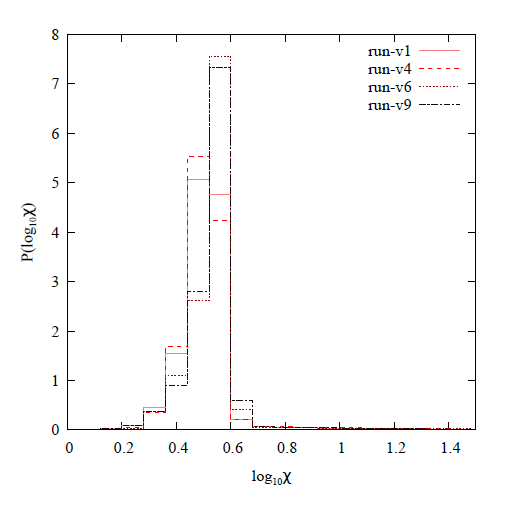
\includegraphics[scale=0.4,angle=0]{figures/fig5_old.png}
\caption{...}
\label{fig:hists}
\end{figure}

\begin{figure}
 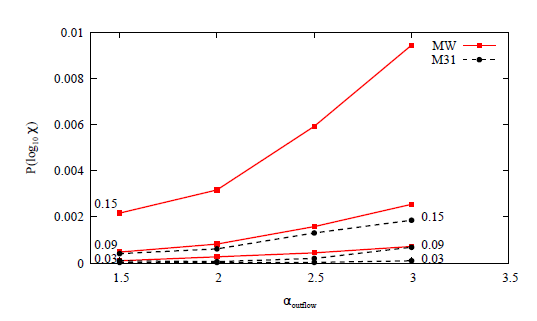
\includegraphics[scale=0.4,angle=0]{figures/fig6_old.png}
 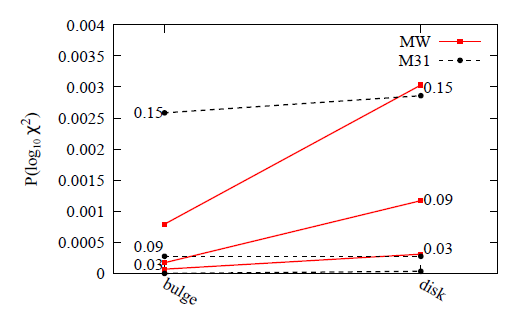
\includegraphics[scale=0.4,angle=0]{figures/fig7_old.png}
 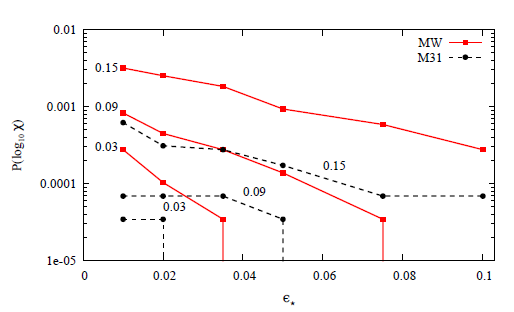
\includegraphics[scale=0.4,angle=0]{figures/fig8_old.png}
\caption{...}
\label{fig:fded}
\end{figure}


As it was shown in section \ref{sec:strategy} we look for galaxies
similar to MW and Andromeda through the us of the distance measure
\ref{eq:distance}. Figure \ref{fig:hists} shows the distribution of
values of $d$. As it can be seen, the distribution is peaked at a
value of $log_{10}(d)\sim 0.4 to 0.5$ depending on the parameter set
used to run the galaxy population. This clearly indicates that there
is a large probability for a galaxy in our samples to be at a distance
in parameter space of that value, meaning that the dominating
population of galaxies (in the mass range explored in this work) is
clearly not a MW or Andromeda-like galaxy. Considering that galaxies
similar to LG galaxies are those with the lowest values of $d$, the
distributions also show that being a LG galaxy is not so probable.

Indeed, in figure \label{fig:fded} we show the associated estimated
probability for a galaxy to be LG galaxy as a function of the model
parameters for a given value of $d$ for the smallest bins in $d$ from
figure \ref{fig:hists}. As it can be clearly seen $P(d)$ grows with
$d$, as expected from figure, but the change depends strongly on the
selection of the value of the model parameters. In particular, it can
be seen that for a given value of $d$ larger values of the
$\alpha_{outflow}$ (runs A1, A2, A3, E5) parameter tend to
maximise $P(d)$, that is, it is going to be more probable to have
LG-like galaxies if a large value of $\alpha_{outflow}$ is used. It is
also interesting to note how, for the largest $d$ bin shown in
figure \label{fig:fded}-top, the probability for a galaxy to be a
MW-like is larger that the one for a galaxy to be a Andromeda-like
galaxy, and the dependence on $\alpha_{outflow}$ is clearly stronger.

A similar behaviour can be seen for the same three $d$-bins when
variating the place where the mass goes to after a merger (bulge or
disk, runs D1 and B1). One can see that there is a clear dependence on
the probability for a galaxy to be LG-like as a function of this
parameter. In particular, choosing that after a merger mass flows to
the disk instead of the spheroid maximises the probability for them to
be LG-like galaxies. Again this dependence is stronger for the MW
than for Andromeda.

A similar trend can be seen exploring the variation of the probability
for a galaxy to be a LG-like as a function of the parameter
$\epsilon_{\star}$ (runs E1, E2, E3, E4, E5). In this case the maximum
value of $P(d)$ is obtained for the lowest values of
$\epsilon_{\star}$, meaning that for the LG galaxies, it ts more
convenient to model the star formation process with a low star
formation efficiency.

In the three panels of figure \label{fig:fded} can also be seen as a
general trend that for a given $d$-bin, and a fixed value of the
parameters, the probability for a galaxy to be a MW-like is larger than
for them to be an Andromeda-like galaxy.

In general, according to the observational constraints, LG galaxies
are favoured by model parameters given by $\alpha_{outflow} \sim 3$,
$\epsilon_{\star} \sim 0.01$ and preferentially leaving the gas and
stars in the disk after mergers.

%answer this question: what does it means that LG-like galaxies are
%more probable if alpha_outflowe is larger? what is happening
%physically?

% Physically what does it means that the probability for a galaxy to
%be LG-like is larger is gas flows to disk after merger than to a
%bulge?

%% the same question for eps_star

\begin{figure}
 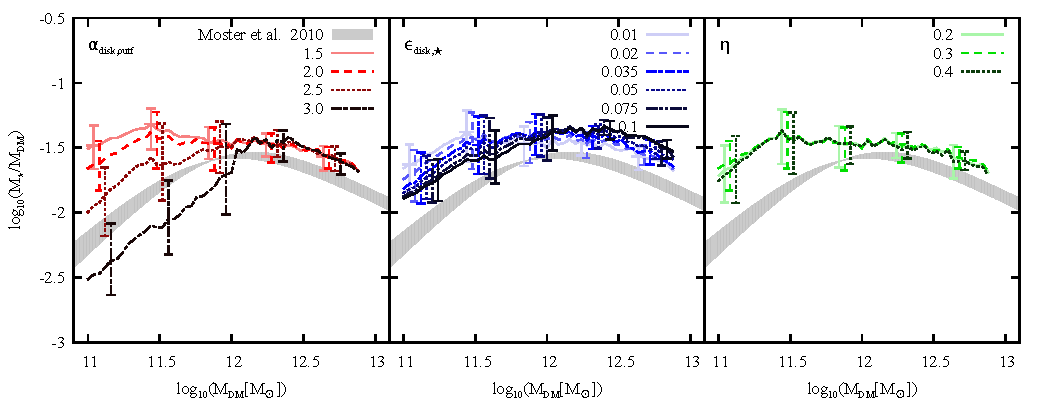
\includegraphics[scale=0.45,angle=0]{figures/runs/run-v1-13-multiplot-star-frac.pdf}
 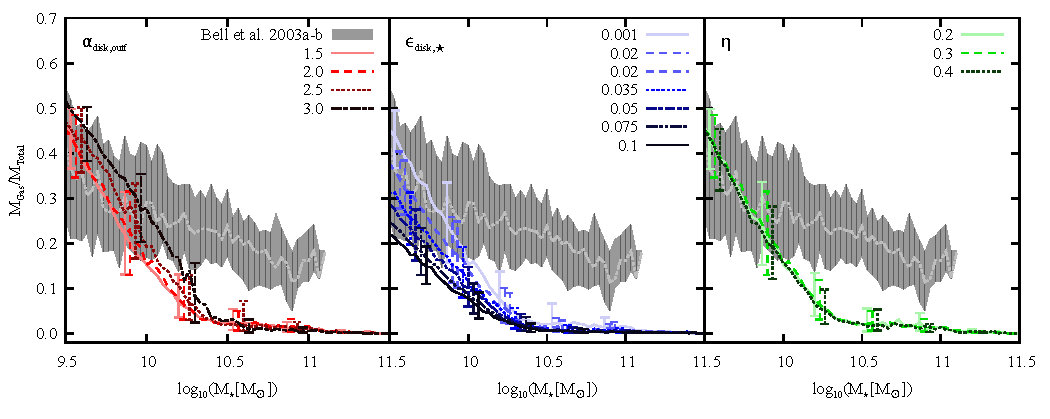
\includegraphics[scale=0.45,angle=0]{figures/runs/run-v1-13-multiplot-gas.pdf}
 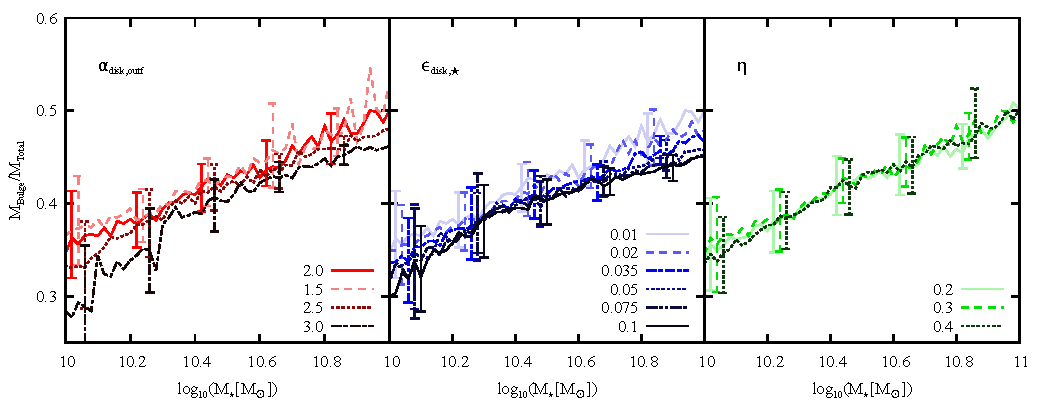
\includegraphics[scale=0.45,angle=0]{figures/runs/run-v1-13-multiplot-bulge.pdf}
\caption{...}
\label{fig:runs}
\end{figure}

One might ask that in general the model parameters that are well
suited to fit the observations of the LG galaxies are not necessarily
the ones that are required to describe the general statistical
properties of the galaxy population. To explore the answer to this
question wee explore now the behaviour of different galaxy properties
in our halo samples and compare the results against observations.

Figure \ref{fig:runs} shows a summary of the runs shown in
table \label{tab:runs} and his impact on variations on the parameters
that characterise the galaxies in our definition: Stellar mass - halo
mass fraction as a function of the stellar mass, gas mass to total
ratio and bulge mass to total as a function of stellar mass. In
general we see that in the halo mass regime explored in this work, the
parameters that most affect the distributions are $\alpha_{outflow}$
and $\epsilon_{\star}$. Nevertheless it is intriguing that in the case
of $\alpha_{outflow}$, the value that best fits the results reported
in the literature (Moster \etal 2010) for the general trend in the
stellar-halo mass relation is $\alpha_{outflow} \sim 2.5-2.7$, but the
value of $\alpha_{outflow} \sim 3$ clearly deviates from the expected
at the low mass end. Nevertheless at the region of halo masses pf the
order of $10^{12}$\hMsun it works quite well. The difference of the
curves at lower halo masses should be due to ..... blah blah
bla... (answer this point!).

The same stellar mass-halo mass relation is seen to be not so strongly
affected -in general- by variations on $\epsilon_{\star}$.  it
can be seen that different values of $\epsilon_{\star}$ produce
different stellar mass- halo mass relations, there are not really
drastically different, conversely to what is observed with
$\alpha_{outflow}$. For the specific case of the $\epsilon_{\star}$,
again the value of $\epsilon_{\star}=0.01$ produces the relations more
strongly deviated at the low mass end of the relation, close to the
halo mass we are interested in $10^{12}$\hMsun, this value provides
an acceptable match to the observations.

Finally, as it can be seen in the figure variations on the final end
of the material after merger (bulge or disk) does not really affect
the stellar mass-halo mass relation in a noticeable maner. We can
however observe that in general the stellar mass-halo mass relation we
produce (even with the reference parameter values) is in general
relatively high.

Not so nice results are obtained for the gas to total mass ratio or
the bulge to total mass ratio as a function of stellar mass. In
general the scatter on the data is high enough to fit with almost all
models on that mass regime below $10^{10.5}$\Msun. In general we see
again that $\epsilon_{\star}$ and $\alpha_{outflow}$ parameter are the
ones that induce noticeable differences in the mean value for the
relations. Large values of $\alpha_{outflow}$ produce slightly more
gas rich galaxies and simultaneously low mass bulges, while low
$\epsilon_{\star}$ values produce galaxies with slightly more mass in
gas and simultaneously larger bulge mass. Variations on the final
fate of the material after merger, bulge or disk, again produce no
major difference on the relations for the models. Despite the
differences observed in the different runs with different model
parameters, all results are equally compatible with observations in
the stellar mass regime below $10^{10}$\Msun, although lower values
of $\epsilon_{\star}$ produce mean quantities closer to observations.

After this exercise we see that in general the value parameters we
obtain as those that maximise the probability of a galaxy to be a
milky way are also well suited to describe statistical the observables
and might represent a valid region in the volume of parameter space
reproducing the properties of the galaxy distribution, implying that
no fictitious assumption must be made to maximise the number of
LG-like galaxies.

\subsection{The LG candidates}

\begin{figure}
 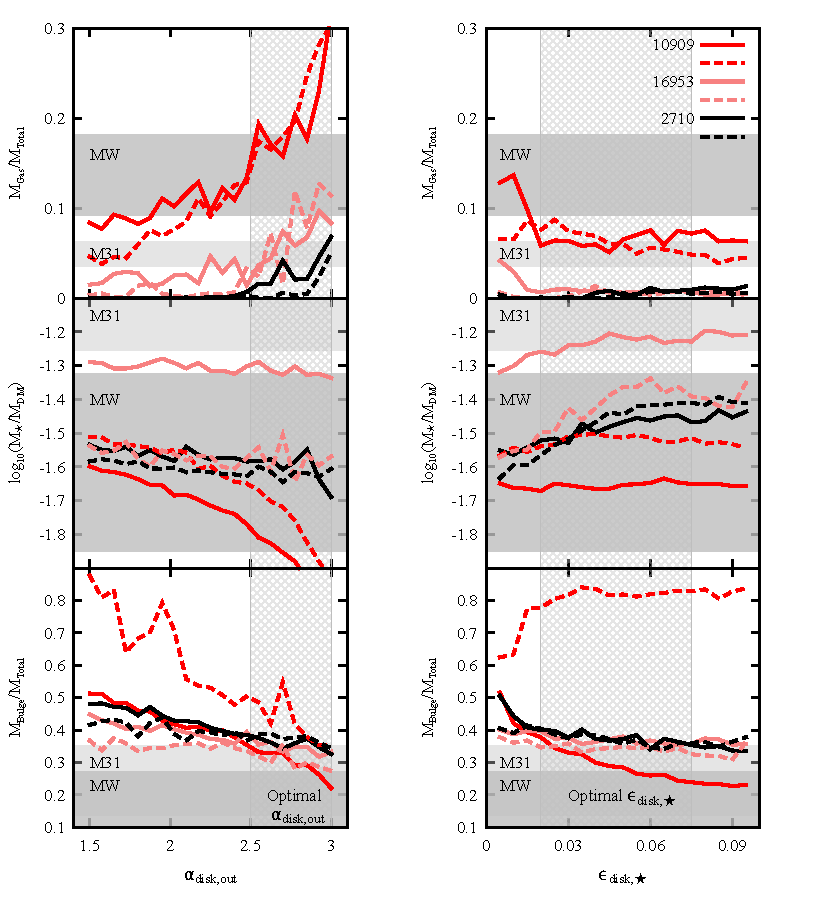
\includegraphics[scale=0.7,angle=0]{figures/LG/LG-props-params-multi-v2.pdf}
\caption{...}
\label{fig:runCands}
\end{figure}


Now we focus our attention on the candidates to MW and Andromeda
galaxy in our constrained simulations and study how the properties of
these galaxies change under variations of the model parameters. From
the simulations we took the merger trees of these two galaxies and ran
our models several times variating smoothly the values of the
parameters $\epsilon_{\star}$ and $\alpha_{outflow}$ and check how the
galaxy properties change under such variations. In order to account for
the variance on the results, we have run, for each galaxy, for each
value of the parameters 100 realisations of the same run and from that
set we compute the median value of the galaxy properties that are
presented in figure \ref{fig:runCands}.

In Figure \ref{fig:runCands} we show the different galaxy properties:
gas to total mass fraction, stellar to total mass fraction and bulge
to total mass fraction all as a function of the values of the
parameters $\epsilon_{\star}$ and $\alpha_{outflow}$ that we have seen
are the ones that affect more strongly the properties of the
distribution of galaxies. The different lines in that figure are
associated to the different galaxy (MW or Andromeda) and to the
different boxes, since we have three different realisations providing
three pairs of candidates.

The horizontal shaded regions indicate the regions where the
observations place the MW and Andromeda galaxies (CITATIONS). The
width of the region is associated with the error bars of the
measurements. The vertical semi-shaded areas indicate the regions in
parameter space that we have found to be those that maximise the
probability of a galaxy to be a LG-like galaxy. The interception of
those two regions would place the region where our MW and Andromeda
candidates are actually fitting our requirements.

A perfect MW or Andromeda galaxy model should be one for which the
lines describing the dependence of the properties on the parameters
intersects the regions of overlaping in all three
properties. Nevertheless that is not the case for our
simulations. According to figure \ref{fig:runCands}-left none of the
models are in agreement with the optimal parameter values. As it can
be seen the LG-galaxies in our simulation 10909 fall in the region of
optimal parameters for the gas mass fraction and.... ESTO ES
CASPA.... ESTO HAY QUE REPETIRLO... QUI HAY ALGO MALO!

%% HACER ESTE EXPERIMENTO: CORRER LAS DISTRIBUCIONES DE CHI Y DEMAS
%% ELIMINANDO UNO DE LOS PARAMETROS PARA EXPLORAR LA DISPERSION
%% ALREDOR DE LAS CURVAS DE CHI. ES DECIR, ES COMO HACER
%% JACK-KNIFE. sE CORREN LAS COSAS CON LA METRICA SIN USAR LA
%% VELOCIDAD CIRCULAR, OTRO RUN SIN EL COLOR, OTRO RUN SIN LA MASA DEL
%% DISCO, ETC. SI LA DEFICION DE ETA ES ESTABLE, DEBERIAN SER TODAS
%% SIMILARES, Y LAS VARIACIONES DEBERIAN SER PEQUEÑAS, MOSTRANDO QUE
%% LA DEFINICION DE DISTANCE MEASURE ES ESTABLE.






%%%%%%%%%%%%%%%%%%%%%%%%%%%%%%%%%%%%%%%%%%%%%%%%%%%%%%%%%%%%%%%%%%%%%%%
%%%%%%%%%%%%%%%%%%%%%%%%%%%%%%%%%%%%%%%%%%%%%%%%%%%%%%%%%%%%%%%%%%%%%%%


\section{Summary and discussion}

 
\section*{Acknowledgments}

The authors wants to tanks to DAAD and Colciencias for the financial
suport through the bilateral colaboration PPP-PROCOL. Project
XXXXXXXX. J.C.M., J.F. and S.G. akcnowledge the hospitality from
Universidad de Antuioquia. S.S. and J.Z. akcnowledge the hospitality
of the Leibniz Institut F\"{u}r Astrophysik Potsdam.

%%%%%%%%%%%%%%%%%%%%%%%%%%%%%%%%%%%%%%%%%%%%%%%%%%%%%%%%%%%%%%%%%%%%%%%
%%%%%%%%%%%%%%%%%%%%%%%%%%%%%%%%%%%%%%%%%%%%%%%%%%%%%%%%%%%%%%%%%%%%%%%


\begin{thebibliography}{99}

\bibitem[Abazajian et al.(2009)]{2009ApJS..182..543A} Abazajian,
  K.~N., Adelman-McCarthy, J.~K., Ag{\"u}eros, M.~A., et al.\ 2009,
  \apjs, 182, 543

\bibitem[Baldry et al.(2008)]{2008MNRAS.388..945B} Baldry, I.~K.,
  Glazebrook, K., \& Driver, S.~P.\ 2008, \mnras, 388, 945

\bibitem[Berlind et al.(2006)]{2006ApJS..167....1B} Berlind, A.~A.,
  Frieman, J., Weinberg, D.~H., et al.\ 2006, \apjs, 167, 1

\bibitem[Blanton et al.(2003)]{2003ApJ...592..819B} Blanton, M.~R.,
  Hogg, D.~W., Bahcall, N.~A., et al.\ 2003, \apj, 592, 819

\bibitem[Blanton et al.(2005)]{2005AJ....129.2562B} Blanton, M.~R.,
  Schlegel, D.~J., Strauss, M.~A., et al.\ 2005, \aj, 129, 2562

\bibitem[Blanton \& Roweis(2007)]{2007AJ....133..734B} Blanton, M.~R.,
  \& Roweis, S.\ 2007, \aj, 133, 734

\bibitem[Bryan \& Norman(1998)]{1998ApJ...495...80B} Bryan, G.~L., \&
  Norman, M.~L.\ 1998, \apj, 495, 80

\bibitem[Crook et al.(2007)]{2007ApJ...655..790C} Crook, A.~C.,
  Huchra, J.~P., Martimbeau, N., et al.\ 2007, \apj, 655, 790

\bibitem[Croton et al.(2006)]{2006MNRAS.365...11C} Croton, D.~J., Springel, 
V., White, S.~D.~M., et al.\ 2006, \mnras, 365, 11

\bibitem[De Lucia \& Blaizot(2007)]{2007MNRAS.375....2D} De Lucia, G.,
  \& Blaizot, J.\ 2007, \mnras, 375, 2

\bibitem[Koester et al.(2007)]{2007ApJ...660..239K} Koester, B.~P.,
  McKay, T.~A., Annis, J., et al.\ 2007, \apj, 660, 239

\bibitem[Lee et al.(2004)]{2004AJ....127.1811L} Lee, B.~C., Allam,
  S.~S., Tucker, D.~L., et al.\ 2004, \aj, 127, 1811

\bibitem[Merch{\'a}n \& Zandivarez(2005)]{2005ApJ...630..759M}
  Merch{\'a}n, M.~E., \& Zandivarez, A.\ 2005, \apj, 630, 759

\bibitem[Moster et al.(2010)]{2010ApJ...710..903M} Moster, B.~P.,
  Somerville, R.~S., Maulbetsch, C., et al.\ 2010, \apj, 710, 903

\bibitem[Mu{\~n}oz-Cuartas et al.(2011)]{2011MNRAS.417.1303M}
  Mu{\~n}oz-Cuartas, J.~C., M{\"u}ller, V., \& Forero-Romero,
  J.~E.\ 2011, \mnras, 417, 1303

\bibitem[Nichol(2004)]{2004cgpc.symp...24N} Nichol, R.~C.\ 2004,
  Clusters of Galaxies: Probes of Cosmological Structure and Galaxy
  Evolution, 24

\bibitem[Reed et al.(2007)]{2007MNRAS.374....2R} Reed, D.~S., Bower,
  R., Frenk, C.~S., Jenkins, A., \& Theuns, T.\ 2007, \mnras, 374, 2

\bibitem[Sheth \& Tormen(2002)]{2002MNRAS.329...61S} Sheth, R.~K., \&
  Tormen, G.\ 2002, \mnras, 329, 61

\bibitem[Springel et al.(2005)]{2005Natur.435..629S} Springel, V.,
  White, S.~D.~M., Jenkins, A., et al.\ 2005, \nat, 435, 629

\bibitem[Tago et al.(2008)]{2008A&A...479..927T} Tago, E., Einasto,
  J., Saar, E., et al.\ 2008, \aap, 479, 927

\bibitem[Tago et al.(2010)]{2010A&A...514A.102T} Tago, E., Saar, E.,
  Tempel, E., et al.\ 2010, \aap, 514, A102

\bibitem[Tinker et al.(2008)]{2008ApJ...688..709T} Tinker, J.,
  Kravtsov, A.~V., Klypin, A., et al.\ 2008, \apj, 688, 709

\bibitem[Tinker et al.(2011)]{2011arXiv1107.5046T} Tinker, J., Wetzel,
  A., \& Conroy, C.\ 2011, arXiv:1107.5046

\bibitem[Wang et al.(2008)]{2008ApJ...687..919W} Wang, Y., Yang, X.,
  Mo, H.~J., et al.\ 2008, \apj, 687, 919

\bibitem[Wang et al.(2011)]{2011MNRAS.413.1973W} Wang, H., Mo, H.~J.,
  Jing, Y.~P., Yang, X., \& Wang, Y.\ 2011, \mnras, 413, 1973

\bibitem[Warren et al.(2006)]{2006ApJ...646..881W} Warren, M.~S.,
  Abazajian, K., Holz, D.~E., \& Teodoro, L.\ 2006, \apj, 646, 881

\bibitem[Weinmann et al.(2011)]{2011MNRAS.416.1197W} Weinmann, S.~M.,
  Lisker, T., Guo, Q., Meyer, H.~T., \& Janz, J.\ 2011, \mnras, 416,
  1197

\bibitem[Wen et al.(2009)]{2009ApJS..183..197W} Wen, Z.~L., Han,
  J.~L., \& Liu, F.~S.\ 2009, \apjs, 183, 197

\bibitem[Wetzel et al.(2011)]{2011arXiv1107.5311W} Wetzel, A.~R.,
  Tinker, J.~L., \& Conroy, C.\ 2011, arXiv:1107.5311

\bibitem[Yang et al.(2007)]{2007ApJ...671..153Y} Yang, X., Mo, H.~J., van 
den Bosch, F.~C., et al.\ 2007, \apj, 671, 153 

\bibitem[Zandivarez \& Mart{\'{\i}}nez(2011)]{2011MNRAS.415.2553Z}
  Zandivarez, A., \& Mart{\'{\i}}nez, H.~J.\ 2011, \mnras, 415, 2553

\bibitem[Zapata et al.(2009)]{2009MNRAS.394.2229Z} Zapata, T., Perez,
  J., Padilla, N., \& Tissera, P.\ 2009, \mnras, 394, 2229


  
\end{thebibliography}


\bsp

\label{lastpage}

\end{document}
